% You should title the file with a .tex extension (hw1.tex, for example)
\documentclass[11pt]{article}

\usepackage{hyperref}
\usepackage{amsmath}
\usepackage{mathtools}
\usepackage{amssymb}
\usepackage{wrapfig}
\usepackage{fancyhdr}
\usepackage{tikz-qtree}
\usepackage{tikz-qtree-compat}
\usepackage[normalem]{ulem}
\usepackage{tikz}
\usepackage{systeme}
\usepackage{graphicx}
\DeclareMathOperator*{\argmin}{argmin}
\DeclareMathOperator*{\argmax}{argmax}
\usepackage{bm}

\oddsidemargin0cm
\topmargin-2cm     %I recommend adding these three lines to increase the 
\textwidth16.5cm   %amount of usable space on the page (and save trees)
\textheight23.5cm  

\newcommand{\question}[2] {\vspace{.25in} \hrule\vspace{0.5em}
\noindent{\bf #1: #2} \vspace{0.5em}
\hrule \vspace{.10in}}
\renewcommand{\part}[1] {\vspace{.10in} {\bf (#1)}}

\newcommand{\myname}{Sean Bittner}
\newcommand{\myandrew}{srb2201@columbia.edu}
\newcommand{\myhwnum}{12}

\setlength{\parindent}{0pt}
\setlength{\parskip}{5pt plus 1pt}
 
\DeclarePairedDelimiter\abs{\lvert}{\rvert}%
 %
\pagestyle{fancyplain}
\rhead{\fancyplain{}{\myname\\ \myandrew}}

\begin{document}

\medskip                        % Skip a "medium" amount of space
                                % (latex determines what medium is)
                                % Also try: \bigskip, \littleskip

\thispagestyle{plain}
\begin{center}                  % Center the following lines
{\Large Draft of new SC section} \\
Sean Bittner \\
November 4, 2020 \\
\end{center}

\section{Identifying neural mechanisms of flexible task switching} \label{results_SC}
In a rapid task switching experiment \cite{duan2015requirement}, rats were explicitly cued on each trial to either orient towards a visual stimulus in the Pro (P) task or orient away from a visual stimulus in the Anti (A) task (Fig. \ref{fig:SC}a). 
Neural recordings in the midbrain superior colliculus (SC) exhibited two populations of neurons that simultaneously represented both task context (Pro or Anti) and motor response (contralateral or ipsilateral to the recorded side): the Pro/Contra and Anti/Ipsi neurons \cite{duan2018collicular}.
Duan et al. proposed a model of SC that, like the V1 model analyzed in the previous section, is a four-population dynamical system.  
We analyzed this model, where the neuron-type populations are functionally-defined as the Pro- and Anti-populations in each hemisphere (left (L) and right (R)), their connectivity is parameterized geometrically  (Fig. \ref{fig:SC}B).
The input-output function of this model is chosen such that the population responses $\mathbf{x} = [x_{LP}, x_{LA}, x_{RP}, x_{RA}]^\top$ are bounded from 0 to 1 as a function $f$ of a dynamically evolving internal variable $\mathbf{u}$.
The dynamics evolve with timescale $\tau=0.09$ governed by connectivity weights $W$
\begin{equation}
\begin{split}
\tau \frac{d\mathbf{u}}{dt} &= -\mathbf{u} + W\mathbf{x} + \mathbf{h} + \epsilon d\mathbf{B} \\
\mathbf{x} &= f(\mathbf{u})
\end{split}
\end{equation}
with white noise of variance $\epsilon^2 = 0.2^2$.
The input $\mathbf{h}$ is comprised of a cue-dependent input to the Pro or Anti populations, a stimulus orientation input to either the Left or Right populations, and a choice-period input to the entire network (see Section \ref{methods_SC}).
Here, we use EPI to determine the changes in network connectivity $\mathbf{z} = [sW, vW, dW, hW]^{\top}$ resulting in execution of rapid task switching behavior.

\begin{figure}
\begin{center}
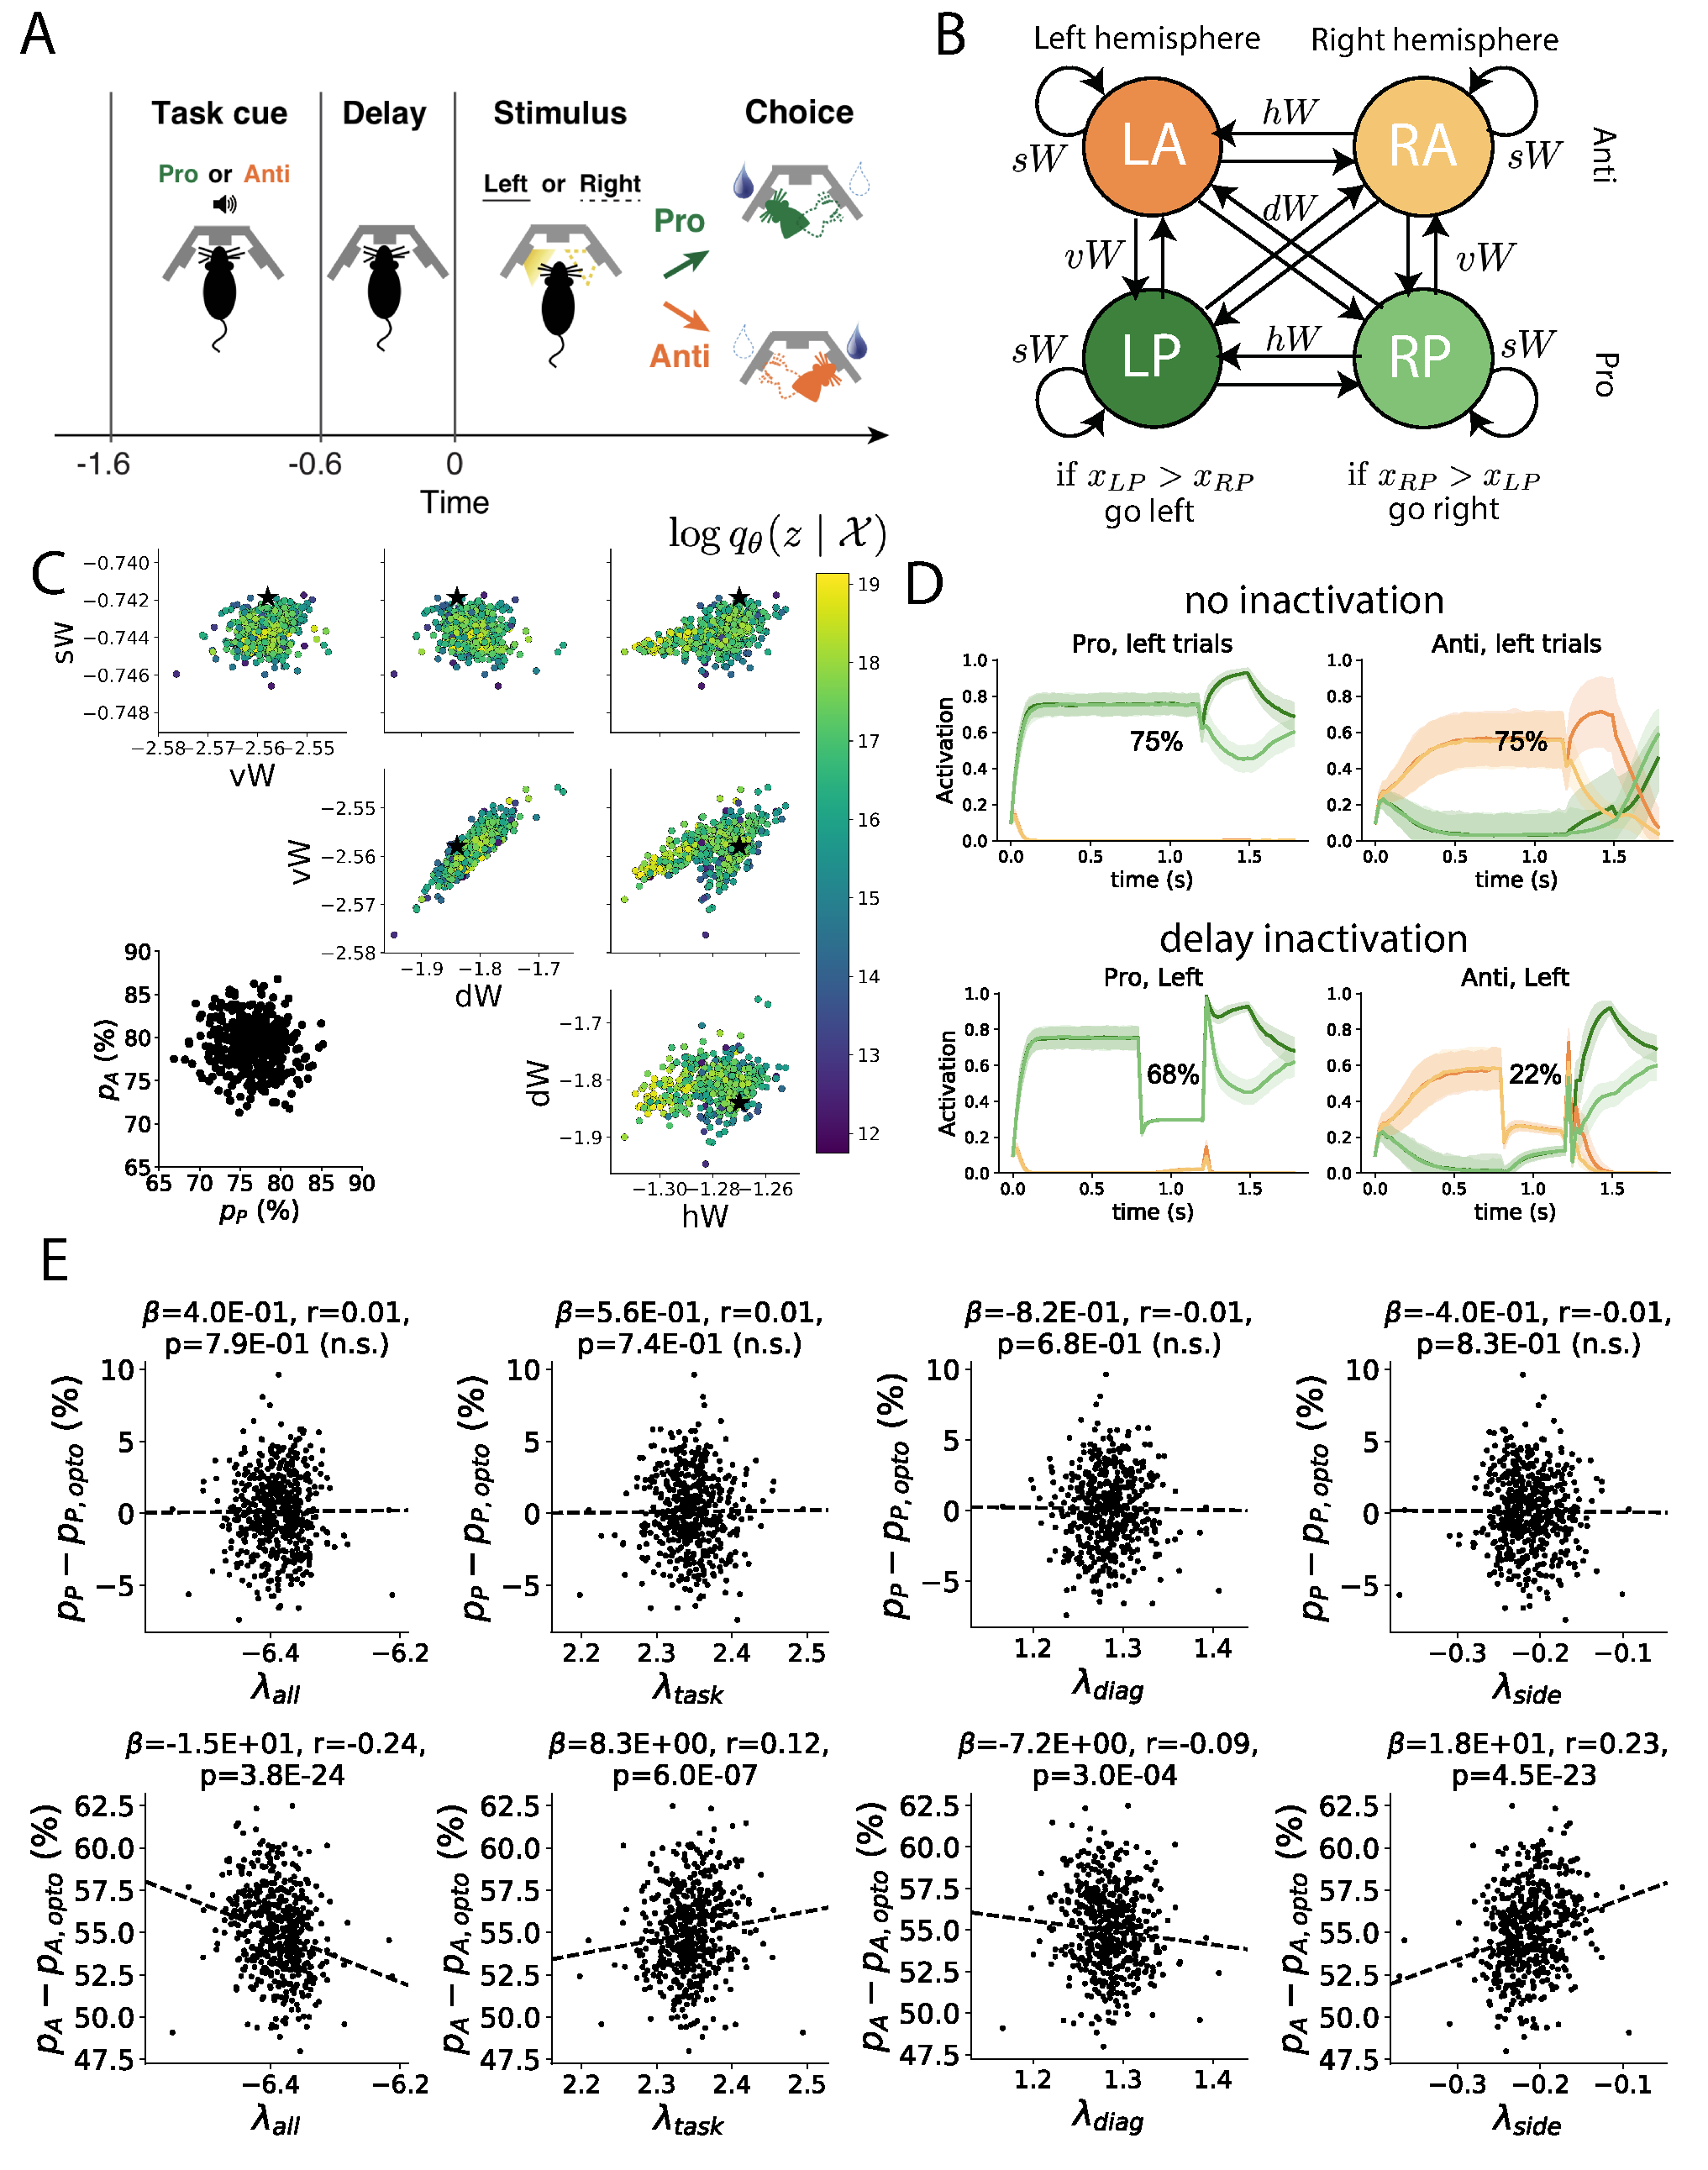
\includegraphics[scale=0.5]{figs/fig4.pdf}
\end{center}
\caption{\small EPI reveals changes in SC \cite{duan2018collicular} connectivity that control task accuracy.  
A. Rapid task switching behavioral paradigm (see text). 
B. Model of superior colliculus (SC). Neurons: LP - left pro, RP - right pro, LA - left anti, RA - right anti. 
Parameters: $sW$ - self, $hW$ - horizontal, $vW$ -vertical, $dW$ - diagonal weights.  
Subscripts $P$ and $A$ of connectivity weights indicate Pro or Anti populations, and e.g. $vW_{PA}$ is a vertical weight from an Anti to a Pro population.  
C. The Schur decomposition of the weight matrix $W = V\Lambda V^{-1}$ is a unique decomposition with orthogonal $V$ and upper triangular $\Lambda$. Schur modes: $v_{\text{all}}$, $v_{\text{task}}$, $v_{\text{side}}$, and $v_{\text{diag}}$.  
D. The marginal EPI distributions of the Schur eigenvalues at each level of task accuracy.
E. The correlation of Schur eigenvalue with task performance in each learned EPI distribution.}
\label{fig:SC}
\end{figure}

We define rapid task switching behavior as accurate execution of each task.  Inferred models should not exhibit fully random responses (50\%), or perfect performance (100\%), since perfection is never attained by even the best trained rats.
We formulate rapid task switching as an emergent property by stipulating that the average accuracy in the Pro task $p_P(\mathbf{x}, \mathbf{z})$ and Anti task $p_A(\mathbf{x}, \mathbf{z})$ be $75\%$ with variance $5\%^2$.
\begin{equation}\label{eq:EP}
\begin{split}
\mathcal{X} ~~:~~ \mathbb{E}_{\mathbf{z}}\begin{bmatrix} p_P(\mathbf{x}; \mathbf{z}) \\ p_A(\mathbf{x}; \mathbf{z}) \end{bmatrix}  &~~=~~  \begin{bmatrix} 75\% \\ 75\% \end{bmatrix}  \\ 
 \text{Var}_{\mathbf{z}}\begin{bmatrix} p_P(\mathbf{x}; \mathbf{z}) \\ p_A(\mathbf{x}; \mathbf{z}) \end{bmatrix}  &~~=~~  \begin{bmatrix} 5\%^2 \\ 5\%^2  \end{bmatrix}
\end{split}
\end{equation}
A variance of $5\%$ performance in each task will confer a posterior producing performances ranging from about $65\%-85\%$, allowing us to examine the properties of connectivity that yield better performance.

We ran EPI to obtain SC model connectivity parameters $z$ producing rapid task switching (Fig. \ref{fig:SC}C).
There is strong pairwise correlation between each parameter of the connectivity matrix.
Shading the distribution by $p_P$, we see that positive shifts in the parameters result in lower accuracy in the Pro task.
Indeed, this difference in accuracy is apparent when we simulate this model for greater parameter values (black star) and lower parameter values (gray star) (Fig. \ref{fig:SC}D). 


To make sense of this inferred distributions, we followed the approach of Duan et al. by decomposing the connectivity matrix $W = V\Lambda V^{-1}$ in such a way (the Schur decomposition) that the basis vectors $v_i$ are the same for all $W$ (Fig. SX). 
These basis vectors have intuitive roles in processing for this task, and are accordingly named the \textit{all} mode - all neurons co-fluctuate, \textit{side} mode - one side dominates the other, \textit{task} mode - the Pro or Anti populations dominate the other, and \textit{diag} mode - Pro- and Anti-populations of opposite hemispheres dominate the opposite pair. 
The corresponding eigenvalues (e.g. $\lambda_{\text{task}}$, which change according to $W$) indicate the degree to which activity along that mode is increased or decreased by $W$. 
We found that $\lambda_{\text{all}}$ is anti-correlated with $p_P$ and $\lambda_{\text{task}}$ is correlated with $p_P$.
TODO interpret further.  Maybe push further on the optogenetics analysis.

\section{Supplementary}\label{methods_SC}
\begin{equation}
\mathbf{x}_\alpha = f(\mathbf{u}) = \left(\frac{1}{2}\tanh\left(\frac{\mathbf{u}_\alpha - \epsilon}{\zeta}\right)+ \frac{1}{2} \right)
\end{equation}
where $\epsilon = 0.05$ and $\zeta = 0.5$.  

The accuracies of $p_P$ and $p_A$ are calculated as
\begin{equation}
p_P(\mathbf{x}; \mathbf{z}) = \mathbb{E}_{x \sim p(x \mid z)}\left[\Theta[x_{LP}(t=1.8s) - x_{RP}(t=1.8s)]\right]
\end{equation}
and 
\begin{equation}
p_A(\mathbf{x}; \mathbf{z}) = \mathbb{E}_{x \sim p(x \mid z)}\left[\Theta[x_{RP}(t=1.8s) - x_{LP}(t=1.8s)]\right]
\end{equation}
given that the stimulus is on the left side, where $\Theta$ is the Heaviside step function.

The Heaviside step function is approximated as
\begin{equation}
\Theta(\mathbf{x}) = \text{sigmoid}(\beta \mathbf{x}),
\end{equation}
where $\beta = 100$.

The system receives five inputs throughout each trial, which has a total length of 1.8s.
\begin{equation}
\mathbf{h}(t) = \mathbf{h}_{\text{constant}} + \mathbf{h}_{\text{P,bias}} + \mathbf{h}_{\text{rule}}(t) + \mathbf{h}_{\text{choice-period}}(t) + \mathbf{h}_{\text{light}}(t).
\end{equation}

There are rule-based inputs depending on the condition,
\begin{equation} 
\mathbf{h}_{\text{constant}} = I_{\text{constant}} [1, 1, 1, 1]^\top
\end{equation}
\begin{equation} 
\mathbf{h}_{\text{P,bias}} = I_{\text{P,rule}} [1, 0, 1, 0]^\top
\end{equation}
\begin{equation} \mathbf{h}_{\text{P,rule}}(t) = \begin{cases}
                           I_{\text{P,rule}} [1, 0, 1, 0]^\top,& \text{if } t\leq 1.2s \\
                            0,              & \text{otherwise}
                         \end{cases}
\end{equation}
\begin{equation} \mathbf{h}_{\text{A,rule}}(t) = \begin{cases}
                           I_{\text{A,rule}} [0, 1, 0, 1]^\top,& \text{if } t\leq 1.2s \\
                            0,              & \text{otherwise}
                         \end{cases}
\end{equation}
a choice-period input,
\begin{equation} \mathbf{h}_{\text{choice}}(t) = \begin{cases}
                           I_{\text{choice}} [1, 1, 1, 1]^\top,& \text{if } t > 1.2s \\
                            0,              & \text{otherwise}
                         \end{cases}
\end{equation}
and an input to the right or left-side depending on where the light stimulus is delivered.     
\begin{equation}  \mathbf{h}_{\text{light}}(t) = \begin{cases}
                           I_{\text{light}} [1, 1, 0, 0]^\top,& \text{if } t > 1.2s \text{ and Left} \\
                           I_{\text{light}} [0, 0, 1, 1]^\top,& \text{if } t > 1.2s \text{ and Right} \\
                            0,              & t \leq 1.2s
                         \end{cases} .
\end{equation}
The input parameterization was fixed to $I_{\text{constant}} = 0.75$, $I_{\text{P,bias}} = 0.5 $, $I_{\text{P,rule}} = 0.6$,  $I_{\text{A,rule}} = 0.6$,  $I_{\text{choice}} = 0.25$,  and $I_{\text{light}} = 0.5$.


\begin{figure}
\begin{center}
\includegraphics[scale=0.75]{figs/figSX2.pdf}
\end{center}
\caption{\small Sentence 1 .
A. Rapid task switching behavioral paradigm (see text). 
B. blah}
\label{fig:SC_EPI2}
\end{figure}

\begin{figure}
\begin{center}
\includegraphics[scale=0.75]{figs/figSX1.pdf}
\end{center}
\caption{\small Sentence 1 .
A. Rapid task switching behavioral paradigm (see text). 
B. blah}
\label{fig:SC_Eigs}
\end{figure}



\bibliography{epi}
\bibliographystyle{unsrt}

\end{document}